\documentclass[10pt,t]{beamer}

% fonts
\usefonttheme{professionalfonts}
\usepackage[osf, sc]{mathpazo} % for rm
\usepackage{courier} % for mono
% \usepackage[euler-digits]{eulervm}
\usefonttheme{serif}
% more about eulervm:
% \mathrm -> rmdefault
% \mathbf -> bfdefault
% \mathsf -> sfdefault
% \mathtt -> ttdefault
% Thus, you should redefine the default text fonts before loading the eulervm package!
% redefine: \mathit, \mathbold, \mathcal

%math
\usepackage{amsmath}
\DeclareMathOperator*{\argmin}{arg\,min}
\DeclareMathOperator*{\argmax}{arg\,max}
\newcommand*\diff{\mathop{}\!\mathrm{d}}
% color
\definecolor{brown}{rgb}{0.4, 0.208, 0.192}
\definecolor{gray1}{rgb}{0.125, 0.125, 0.125}
\definecolor{gray2}{rgb}{0.157, 0.157, 0.157}
\definecolor{green2}{rgb}{0.16862745098039217,0.4,0.19607843137254902}
\definecolor{blue2}{rgb}{0,0.40784313725490196,0.6352941176470588}
\definecolor{brown2}{rgb}{0.6235294117647059,0.2901960784313726,0}

\definecolor{blue}{rgb}{0.18, 0.2, 0.529}
\definecolor{orange}{RGB}{206,117,59} % used for strong
\definecolor{green}{RGB}{49,104,108} % used for everywhere, link,...
\definecolor{red}{RGB}{133,60,66}
\definecolor{pink}{RGB}{184,86,150}



\setbeamercolor{caption name}{fg=green}

% settings for itemize and enumerate
\setbeamertemplate{itemize item}{\textbullet}
\setbeamertemplate{itemize subitem}{\bfseries --}
\setbeamertemplate{itemize subsubitem}{$\circ$}
\setbeamercolor{itemize item}{fg=green}
\setbeamercolor{itemize subitem}{fg=brown}
\setbeamercolor{itemize subsubitem}{fg=gray2}

\setbeamertemplate{enumerate item}{\arabic{enumi}.}
\setbeamertemplate{enumerate subitem}{(\roman{enumii})}
\setbeamertemplate{enumerate subsubitem}{\alph{enumiii}.}
\setbeamercolor{enumerate item}{fg=green}
\setbeamercolor{enumerate subitem}{fg=brown}
\setbeamercolor{enumerate subsubitem}{fg=gray2}
% main page style
\setbeamercolor{background canvas}{bg=white}
\setbeamercolor{normal text}{fg=black}
\setbeamertemplate{footline}[frame number]
\setbeamertemplate{navigation symbols}{}
\setbeamercolor{block title}{bg=green!90!black,fg=white}
\setbeamercolor{block body}{bg=green!10}
% frametitle
\setbeamertemplate{frametitle}
{
    \vskip 5pt
    \strut\Large\textcolor{green}{\insertframetitle}\strut
    \ifx\insertframesubtitle\empty
    \vskip-1.7ex
    \textcolor{green}{\hrule height0pt depth0.5pt \relax}
    \else
    \vskip-1ex
    \strut\small\textcolor{green}{\insertframesubtitle}\strut
    \textcolor{green}{\hrule height0pt depth0.5pt \relax}
    \fi
}
% titlepage
\setbeamertemplate{title page}
{
  \makebox[\textwidth][c]{
    \begin{minipage}[b][0.75\paperheight][c]{0.9\textwidth}
      \centering
      \huge\rm\inserttitle\\
      \Large\rm\insertsubtitle
      \vskip-1.5ex
      \textcolor{green}{\hrule height0pt depth0.8pt \relax}
      \vskip5pt
      \rm\normalsize\insertauthor
    \end{minipage}
  }

  \makebox[\textwidth][c]{
    \begin{minipage}[b][0.25\paperheight][c]{0.4\textwidth}
      \centering
      \rm\insertinstitute
      \par
      \rm\insertdate
    \end{minipage}
  }
}

\usepackage{hyperref}

\usepackage{booktabs}
% ********************************************************************
% tikz
% ********************************************************************
\usepackage{tikz}
\usetikzlibrary{positioning}
\usetikzlibrary{decorations.markings}
\usepackage{pgfplots}






\title{Empirical Asset Pricing \\ Problem Set $2$}
\author{Yu Zhou, HKUST}
\date{\today}


\begin{document}

\maketitle

\begin{frame}{Q1: Return decompostition}
\begin{itemize}
  \item Log-linear approximation of return:
  \begin{equation*}
  \begin{split}
  & r_{t+1} = \rho pd_{t+1} - pd_t + \Delta d_{t+1} \\
  & E_t[r_{t+1}] = \rho E_t[pd_{t+1}] - pd_t + E_{t}[\Delta d_{t+1}]
  \end{split}
  \end{equation*}
  \item Taking difference between realized return and expected return, we can obtain unexpected return:
  \begin{equation*}
  \begin{split}
  & r_{t+1} - E_t[r_{t+1}] \\
  = & (E_{t+1} - E_{t}) [\rho pd_{t+1}] + (E_{t+1} - E_{t}) [\Delta d_{t+1}] \\
  = & (E_{t+1} - E_{t}) \bigg[\sum_{j = 1}^{\infty} \rho^{j} (\Delta d_{t+1+j} - r_{t+1+j})\bigg] + (E_{t+1} - E_{t}) [\Delta d_{t+1}] \\
  = & \underbrace{(E_{t+1} - E_{t}) \bigg[\sum_{j = 0}^{\infty} \rho^{j} \Delta d_{t+1+j}\bigg]}_{\text{cash-flow shocks/news}} - \underbrace{(E_{t+1} - E_{t}) \bigg[\sum_{j = 1}^{\infty} \rho^{j} r_{t+1+j}\bigg]}_{\text{expected-return shocks/news}}
  \end{split}
  \end{equation*}
  \item Cash-flow news include news of both expected and contemporaneous cash flow.
\end{itemize}
\end{frame}

\begin{frame}{Q1: Return decompostition (cont'd)}
\begin{itemize}
  \item Suppose $X_t = (r_t, pd_t)^T \sim VAR(1)$ where $X_{t+1} = AX_{t} + v_{t+1}$. Then, unexpected return turns to be:
  \begin{equation*}
  r_{t+1} - E_t[r_{t+1}] = e_1^T (AX_t + v_{t+1}) - e_1^T AX_t = e_1^T v_{t+1}
  \end{equation*}
  \item The expected-return shocks/news can be expressed as
  \begin{equation*}
  \begin{split}
  Nr & = (E_{t+1} - E_{t}) \bigg[\sum_{j = 1}^{\infty} \rho^{j} r_{t+1+j}\bigg] \\
  & = \sum_{j = 1}^{\infty} \rho^{j} e_1^T (A^j X_{t+1} - A^{j+1} X_{t}) \\
  & = e_1^T \sum_{j = 1}^{\infty} \rho^{j} A^j v_{t+1} \\
  & = e_1^T \sum_{j = 0}^{\infty} \rho^{j} A^j \rho A v_{t+1} \\
  & = \rho e_1^T G v_{t+1}, \text{ where } G = (I - \rho A)^{-1}A
  \end{split}
  \end{equation*}
\end{itemize}
\end{frame}

\begin{frame}{Q1: Return decompostition (cont'd)}
\begin{itemize}
  \item The cash-flow shocks/news can be backed out:
  \begin{equation*}
  Nc = e_1^T(I + \rho G) v_{t+1}
  \end{equation*}
\end{itemize}
\end{frame}






\begin{frame}{Q2: Backing out approach}
\begin{itemize}
  \item Suppose the state variables $X_t = (r_t, pdt)^T$ follows a $VAR(1)$ process where $X_{t+1} = A_0 + A X_{t} + \varepsilon$.
  \begin{itemize}
    \item The long-run expected returns is given by $pd_t^r = e1^T G X_t$.
  \end{itemize}
  \item The long-run expected dividend growth can be backed out as
  $$
  pd_{t, \text{indirect}}^{d} = pd_t + pd_t^r
  $$
  \item This is equivalent to $e_d^T G X_t$.
\end{itemize}
\end{frame}





\begin{frame}{Q2: Direct forecast approach}
\begin{itemize}
  \item Dividend growth rates follow a process as
  $$
  \Delta d_{t+1} = b_1 + b^T X_t + u_{t+1}
  $$
  which can be estimated by running an OLS regression.
  \item Then, the long-run expected dividend growth rate can be expressed to be
  \begin{equation*}
  \begin{split}
  pd^{d}_{t, \text{direct}} & = E_{t} \bigg[\sum_{j = 1}^{\infty} \rho^{j - 1} \Delta d_{t+j}\bigg] \\
  & = b^T \sum_{j = 1}^{\infty} \rho^{j - 1} A^{j - 1} X_t \\
  & = b^T (I - \rho A)^{-1}X_t
  \end{split}
  \end{equation*}
\end{itemize}
\end{frame}



\begin{frame}{Q2: Indirect v.s. direct approach}
\begin{figure}[h!]
\centering
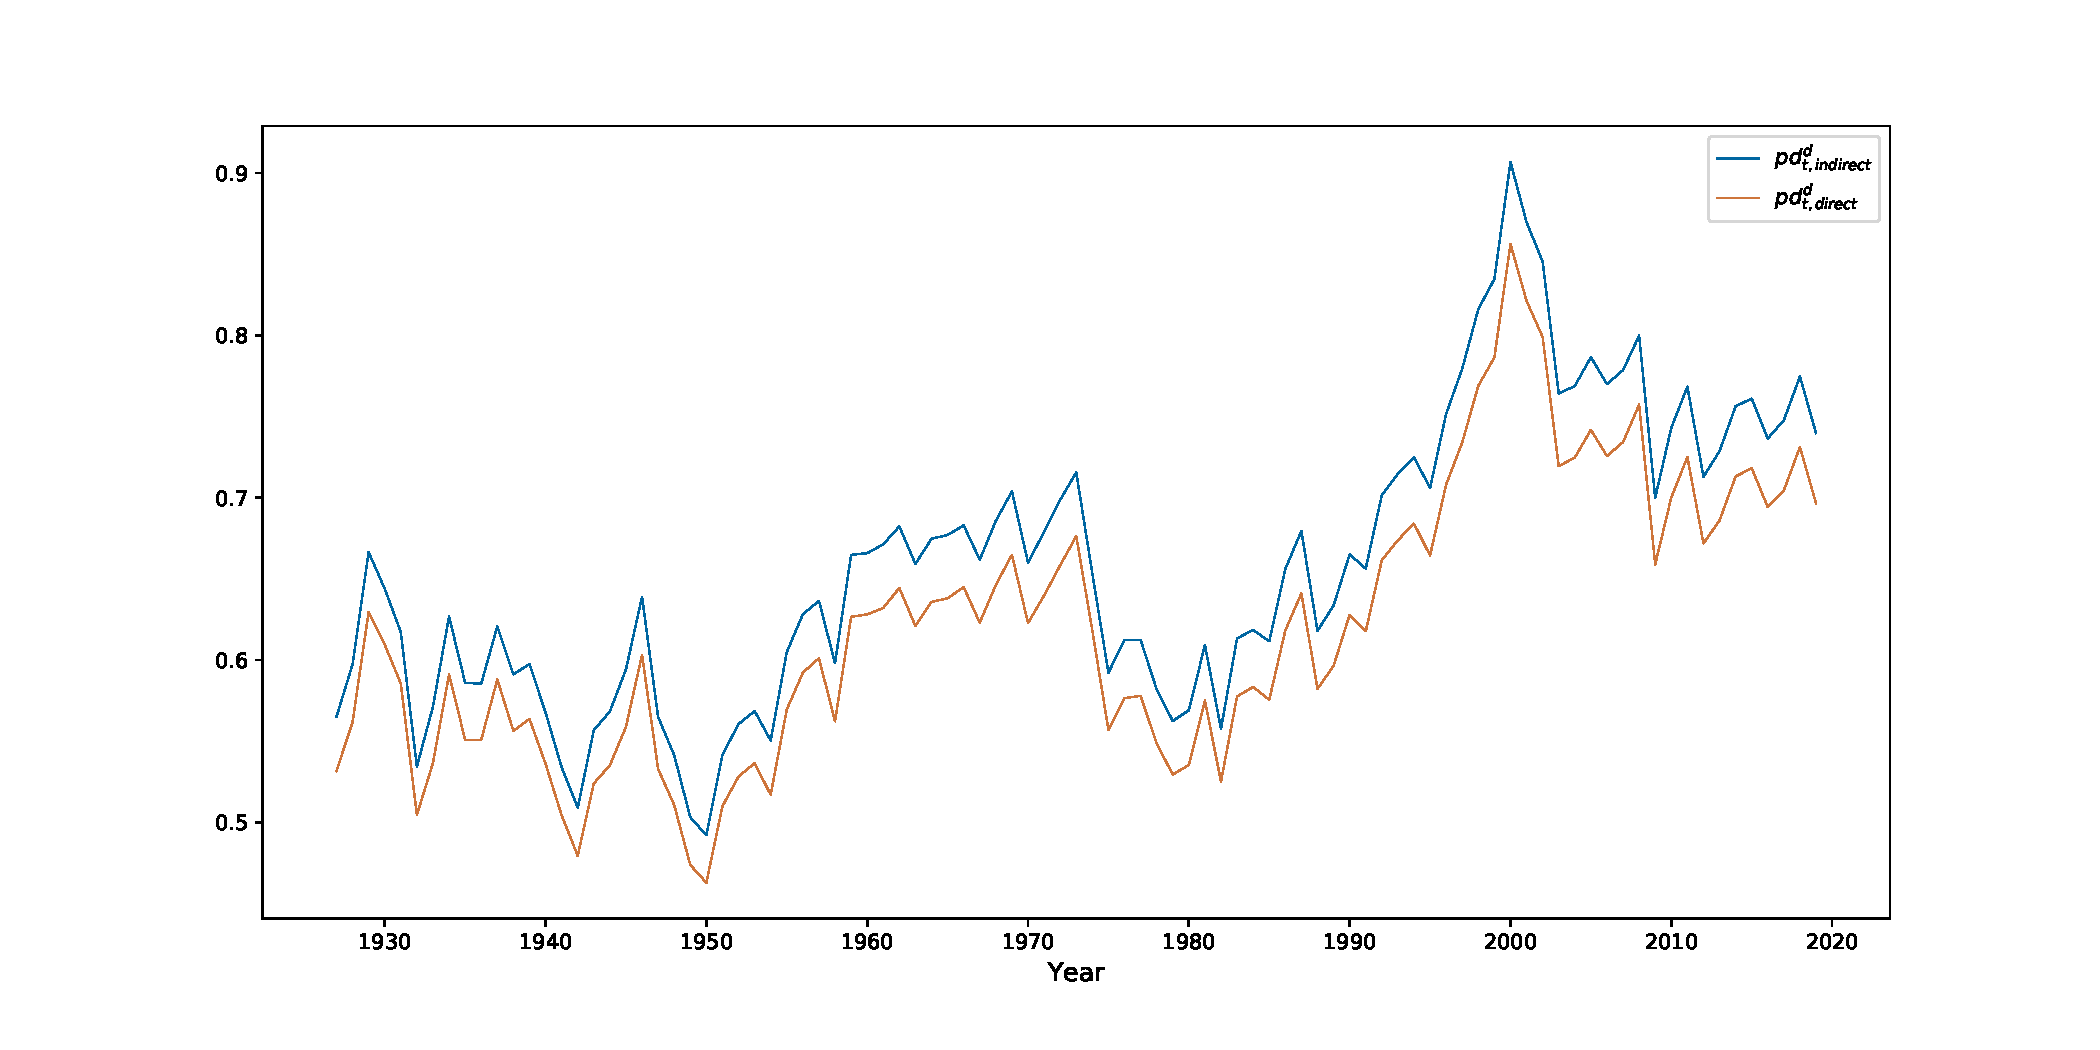
\includegraphics[width=\linewidth]{q2fig1.pdf}
\caption{This figure plots $pd^{d}_{t, \text{direct}}$ and $pd^{d}_{t, \text{indirect}}$ under state variables $X_t = (r_t, pd_t)^T$. As you can see, the backing out approach works well. The reason is that by assuming $r_t$ and $pd_t$ follow $VAR(1)$, log-return identity indicates a linear relation between $\Delta d_{t+1}$ and $X_t$. So backing out approach coincide with direct linear regression of $\Delta d_{t+1}$ on $X_t$.}
\end{figure}
\end{frame}




\begin{frame}{Q2: Different state variables}
\begin{itemize}
  \item Now, re-assuming the state variables used by investors to predict stocks' future performance to be: $X_t = (r_t, \text{term}_t, \text{def}_t)^T$, where 
  \begin{itemize}
    \item $\text{term}_t$ is the difference in long-term and short-term Treasury yield;
    \item $\text{def}_t$ is the difference in yield between corporate bonds and long-term Treasury bonds.
  \end{itemize}
\end{itemize}
\end{frame}

\begin{frame}{Q2: Indirect v.s. direct approach}
\begin{figure}[h!]
\centering
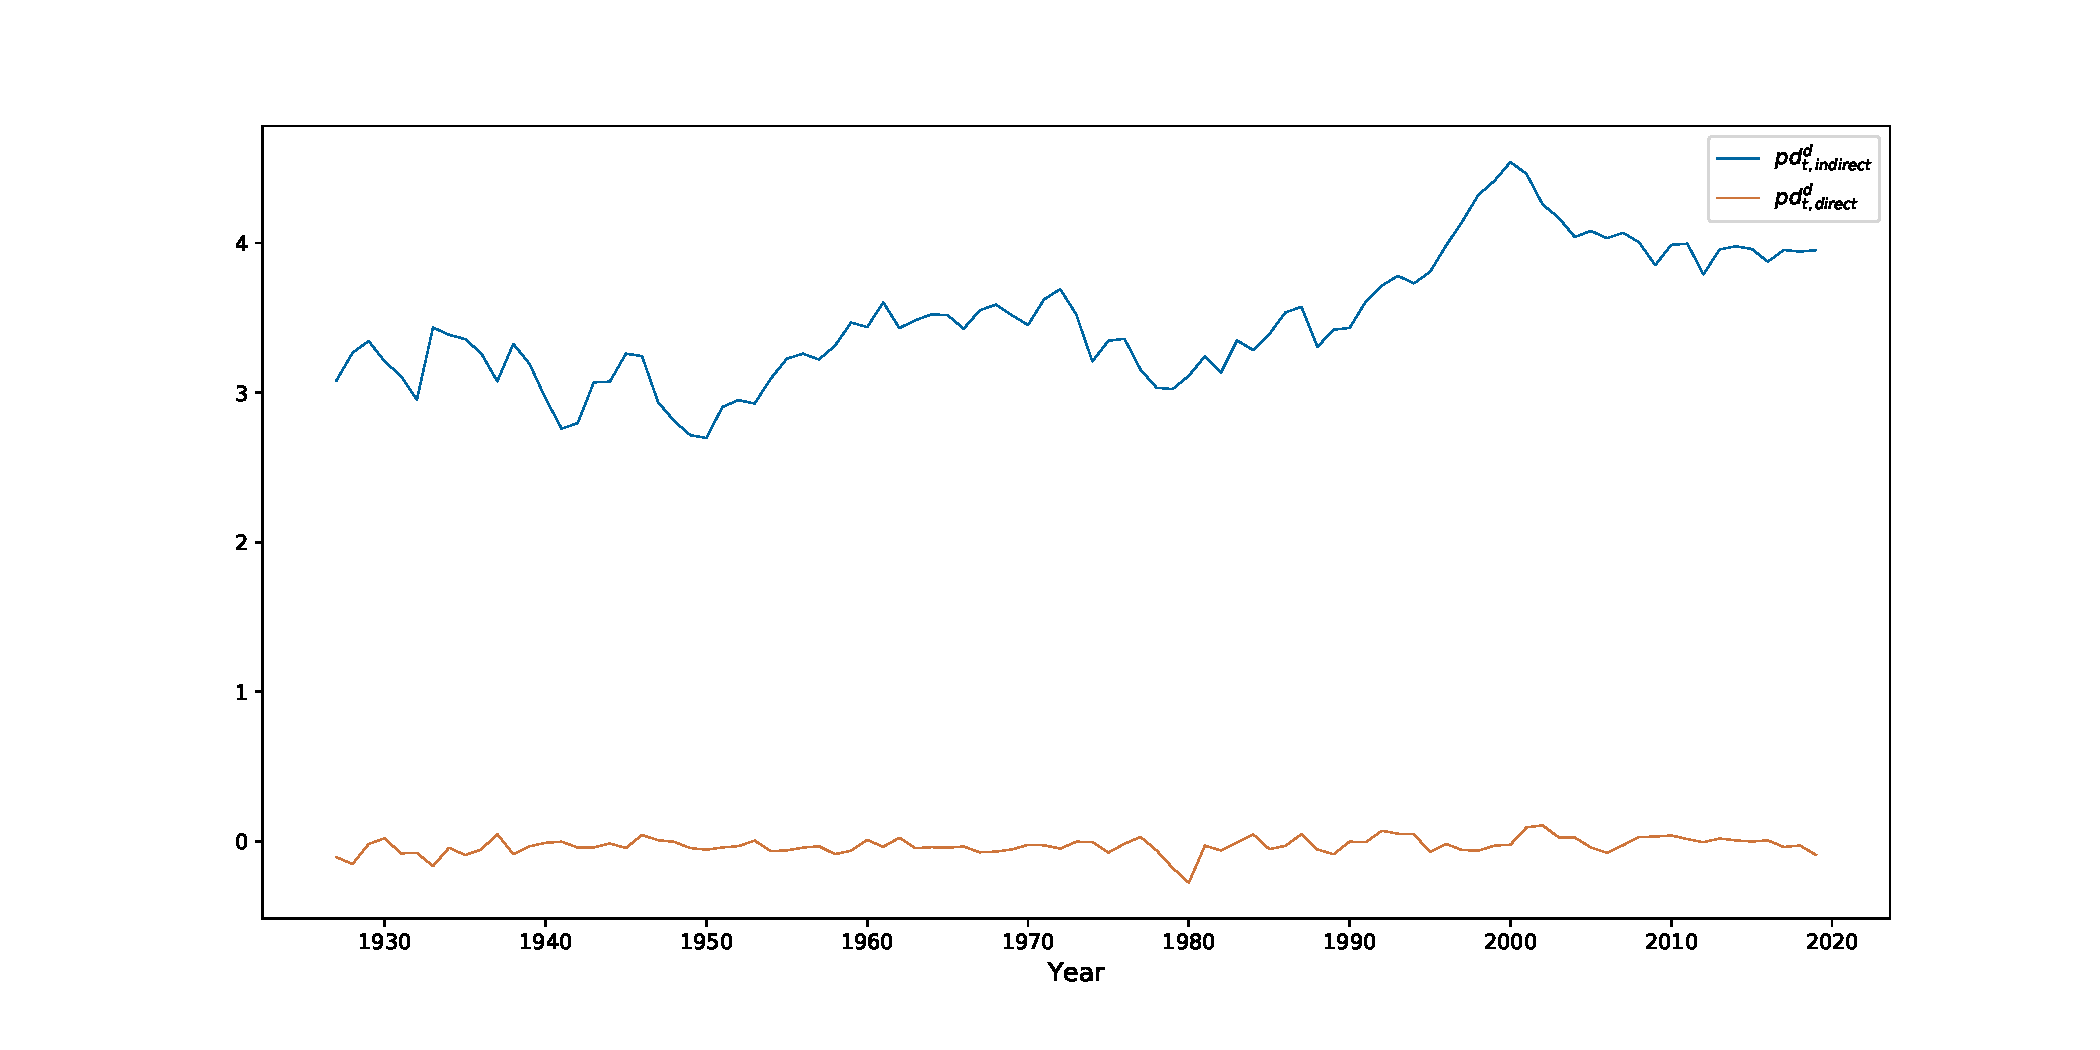
\includegraphics[width=\linewidth]{q2fig2.pdf}
\caption{This figure plots $pd^{d}_{t, \text{direct}}$ and $pd^{d}_{t, \text{indirect}}$ under state variables $X_t = (r_t, \text{term}_t, \text{def}_t)^T$. These approaches work so differently. The reason is that by assuming $r_t$ and $pd_t$ follow $VAR(1)$, log-return identity indicates a linear relation between $\Delta d_{t+1}$ and $\{X_t, pd_{t}\}$. So backing out approach departs from direct linear regression of $\Delta d_{t+1}$ on $X_t$.}
\end{figure}
\end{frame}












\begin{frame}{Q3: Cochrane (2007)}
\begin{itemize}
  \item Suppose a single-state-variable case where $X_{t} = dp_t$. Variables of interest in this world are follows a $VAR(1)$ process:
  \begin{equation*}
  \begin{split}
  r_{t+1} & = a_r + b_r dp_t + \varepsilon_{t+1}^r \\
  \Delta d_{t+1} & = a_d + b_d dp_t + \varepsilon_{t+1}^d \\
  dp_{t+1} & = a_{dp} + \phi dp_t + \varepsilon_{t+1}^{dp} \\
  \end{split}
  \end{equation*}
  \item The log-linear identity $r_{t+1} = - dp_{t+1} + dp_t + \Delta d_{t+1}$ implies the following restrictions (i.e., restricted $VAR(1)$)\footnote{Remark: $dp_t$ is orthogonal to the residual terms}
  \begin{equation*}
  \begin{split}
  b_r &= -\rho \phi + 1 + b_d \\
  \varepsilon_{t+1}^r &= -\rho\varepsilon_{t+1}^{dp} + \varepsilon_{t+1}^d
  \end{split}
  \end{equation*}
\end{itemize}
\end{frame}



\begin{frame}{Q3: Cochrane (2007) (cont'd)}
\vskip1.5cm
\begin{table}
\begin{tabular}{lcccc}
\toprule
& slope & \multicolumn{3}{c}{covariance (scaled by $100$)} \\
\cmidrule{1-5}
$r_{t+1}$ & $0.08$ & $3.7$ & $1.87$ & $-1.9$ \\
$\Delta d_{t+1}$ & $-0.01$ & $1.87$ & $2.06$ & $0.19$\\
$dp_{t+1}$ & $0.94$ & $-1.9$ & $0.19$ & $2.17$\\
\bottomrule
\end{tabular}
\caption{This table reports the estimates for slope coefficients and covariance matrix of residuals.}
\end{table}
\end{frame}







\begin{frame}{Q3: Cochrane (2007) (cont'd)}
\begin{itemize}
  \item Long-run expected return:
  \begin{equation*}
  \begin{split}
  E_{t} \sum_{j = 1}^{\infty} \rho^{j - 1} r_{t+j} & = \sum_{j = 1}^{\infty} \rho^{j - 1} b_r \phi^{j - 1} dp_t + \text{const.}\\
  & = \frac{b_r}{1 - \rho\phi}dp_t + \text{const.} \quad(\text{since } \rho \in (0,1), \vert\phi\vert < 1)
  \end{split}
  \end{equation*}
  \item Long-run dividend growth rate:
  \begin{equation*}
  \begin{split}
  E_{t} \sum_{j = 1}^{\infty} \rho^{j - 1} \Delta d_{t+j} & = \sum_{j = 1}^{\infty} \rho^{j - 1} b_d \phi^{j - 1} dp_t + \text{const.}\\
  & = \frac{b_d}{1 - \rho\phi}dp_t + \text{const.} \quad(\text{since } \rho \in (0,1), \vert\phi\vert < 1)
  \end{split}
  \end{equation*}
\end{itemize}
\end{frame}

\begin{frame}{Q3: Cochrane (2007) (cont'd)}
\begin{itemize}
  \item the sample estimate of the long-run forecasting coefficients:
  \begin{equation*}
  \begin{split}
  & \hat{b}_{r}^{lr} = \frac{\hat{b}_r}{1 - \rho\hat{\phi}} = 0.93 \\
  & \hat{b}_{d}^{lr} = \frac{\hat{b}_d}{1 - \rho\hat{\phi}} = -0.06
  \end{split}
  \end{equation*}
\end{itemize}
\end{frame}

\begin{frame}{Q3: Simulation}
\begin{itemize}
  \item $H_0$: Stock returns are not predictable ($b_r = 0$). So $b_d = \rho \phi - 1 = -0.087$.
  \item Simulation results:
\begin{table}
\begin{tabular}{lccccc}
\toprule
& $b_r$ & $b_d$ & $\phi$ & $b_r^{lr}$ & $b_d^{lr}$ \\
\cmidrule{1-6}
Point estimates & $0.08$ & $-0.01$ & $0.94$ & $0.93$ & $-0.06$ \\
$H_0$ & $0$ & $-0.087$ & $0.94$ & $0$ & $1$\\
Simulation estimates & $0.04$ & $-0.09$ & $0.9$ & $0.26$ & $-0.74$\\
$p$-value & $0.24$ & $0.03$ & $0.18$ & $0.04$ & $0.04$ \\
\bottomrule
\end{tabular}
\caption{This table reports the point estimates, and simulation estimates under the null hypothesis.}
\end{table}
\end{itemize}
\end{frame}

\begin{frame}{Q3: Simulation (cont'd)}
\begin{itemize}
  \item Observations:
  \begin{itemize}
    \item Start with $H_0$ that $b_r = 0$, the simulation estimates bias upward. And this bias is one-half of the point estimate which implies that the bias is large.
    \item The $p$-value of $b_r^{\text{simulated}}$ is $0.24$ which means that under the null hypothesis, our point estimate can realized with probability $0.24>0.05$. Hence, we can not reject the null hypothesis that return is not predictable.
    \item The $p$-value of $b_d^{\text{simulated}}$ is $0.03 < 0.05$. Hence, we reject the null hypothesis that dividend growth is predictable. However, it is impossible that both return and dividend growth are unpredictable.
    \item The $p$-value of $b_r^{lr,\text{ simulated}}$ is $0.04 < 0.05$. Hence, we reject the null hypothesis that return is not predictable.
  \end{itemize}
\end{itemize}
\end{frame}

\begin{frame}{Q3: Simulation (cont'd)}
\begin{figure}[h!]
\centering
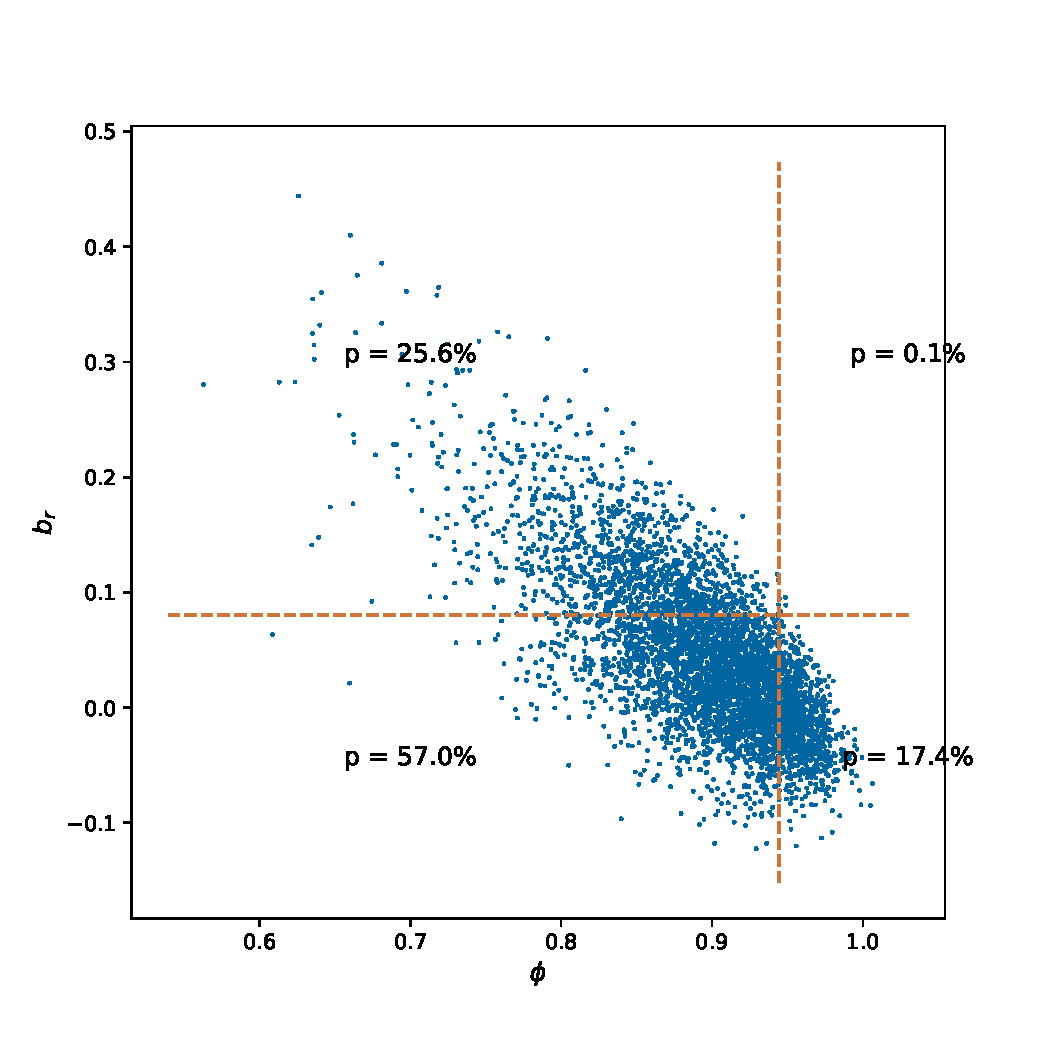
\includegraphics[width=0.5\linewidth]{q3fig1.pdf}
\caption{This figure presents a mechanically negative relation between $\hat{b}_r^{(n)}$ and $\hat{\phi}^{(n)}$. $\hat{b}_r^{(n)}$ is less stable since it decreases corresponding to $\hat{\phi}^{(n)}$. In constract, $\hat{b}_r^{lr, (n)} = \frac{\hat{b}_r^{(n)}}{1 - \rho\hat{\phi}^{(n)}}$ increasing with $\hat{\phi}^{(n)}$ if keeping $\hat{b}_r^{(n)}$ unchanged.}
\end{figure}
\end{frame}




\begin{frame}{Q4: Out-of-sample regressions}
\begin{figure}[h!]
\centering
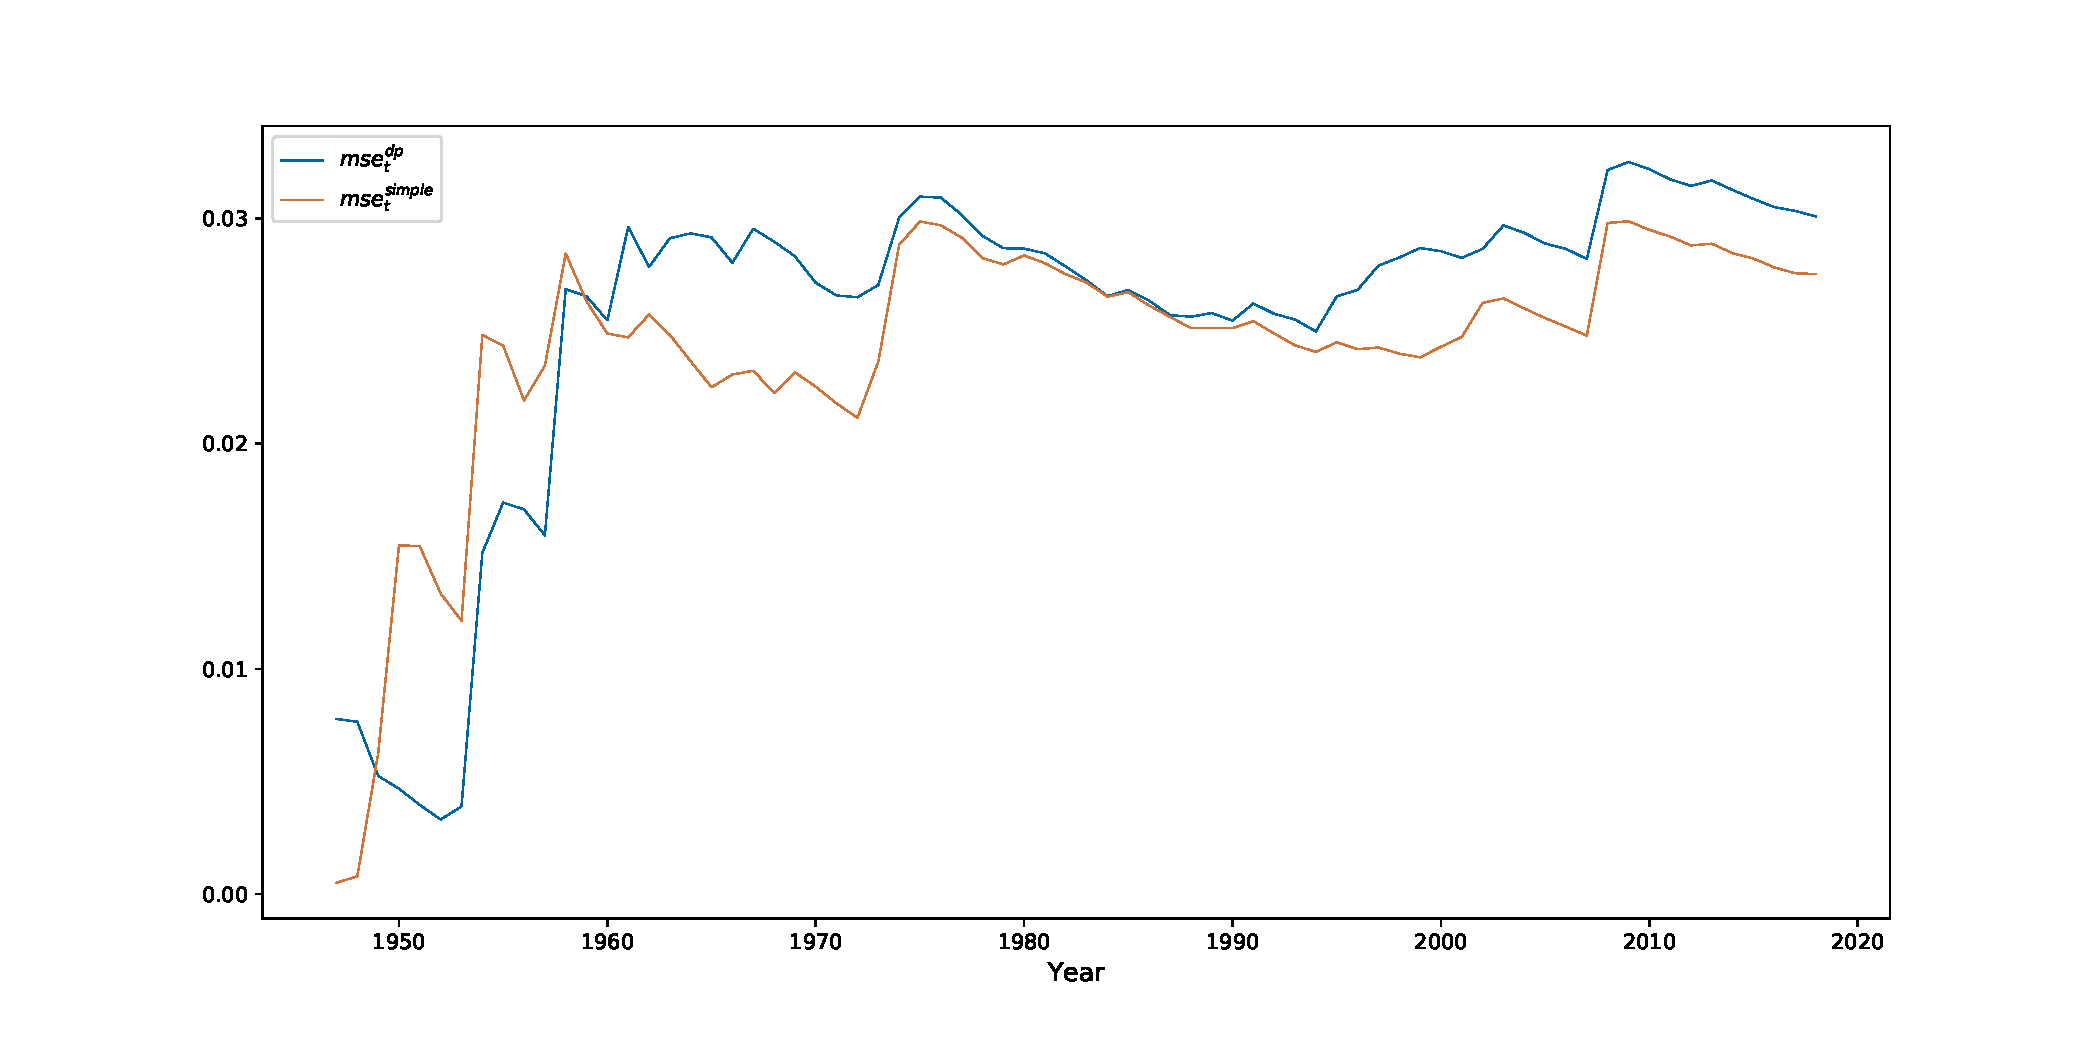
\includegraphics[width=\linewidth]{q4fig1.pdf}
\caption{In the 1950s, the mean-squared errors of these two model increase sharply due to the fact that only few observations are used in in-sample regression. After 1960, the $dp$ model perform poorly relatively to the simple model.}
\end{figure}
\end{frame}



\begin{frame}{Q4: Out-of-sample regressions (cont'd)}
\begin{itemize}
  \item $OOSR^2 = 1 - \frac{\text{MSE}^{dp}_T}{\text{MSE}^{\text{simple}}_T} = -0.093 < 0$. The negative out-of-sample $R^2$ for the $dp$-model implies that sample trading strategy beats the trading strategy based on $dp$.
\end{itemize}
\end{frame}

\begin{frame}{Q4: Simulation}
\begin{itemize}
  \item $H_0$: Dividend growth rates are not predictable ($b_d = 0$). So $b_r = 1 - \rho \phi = 0.087$.
\end{itemize}
\begin{figure}[h!]
\centering
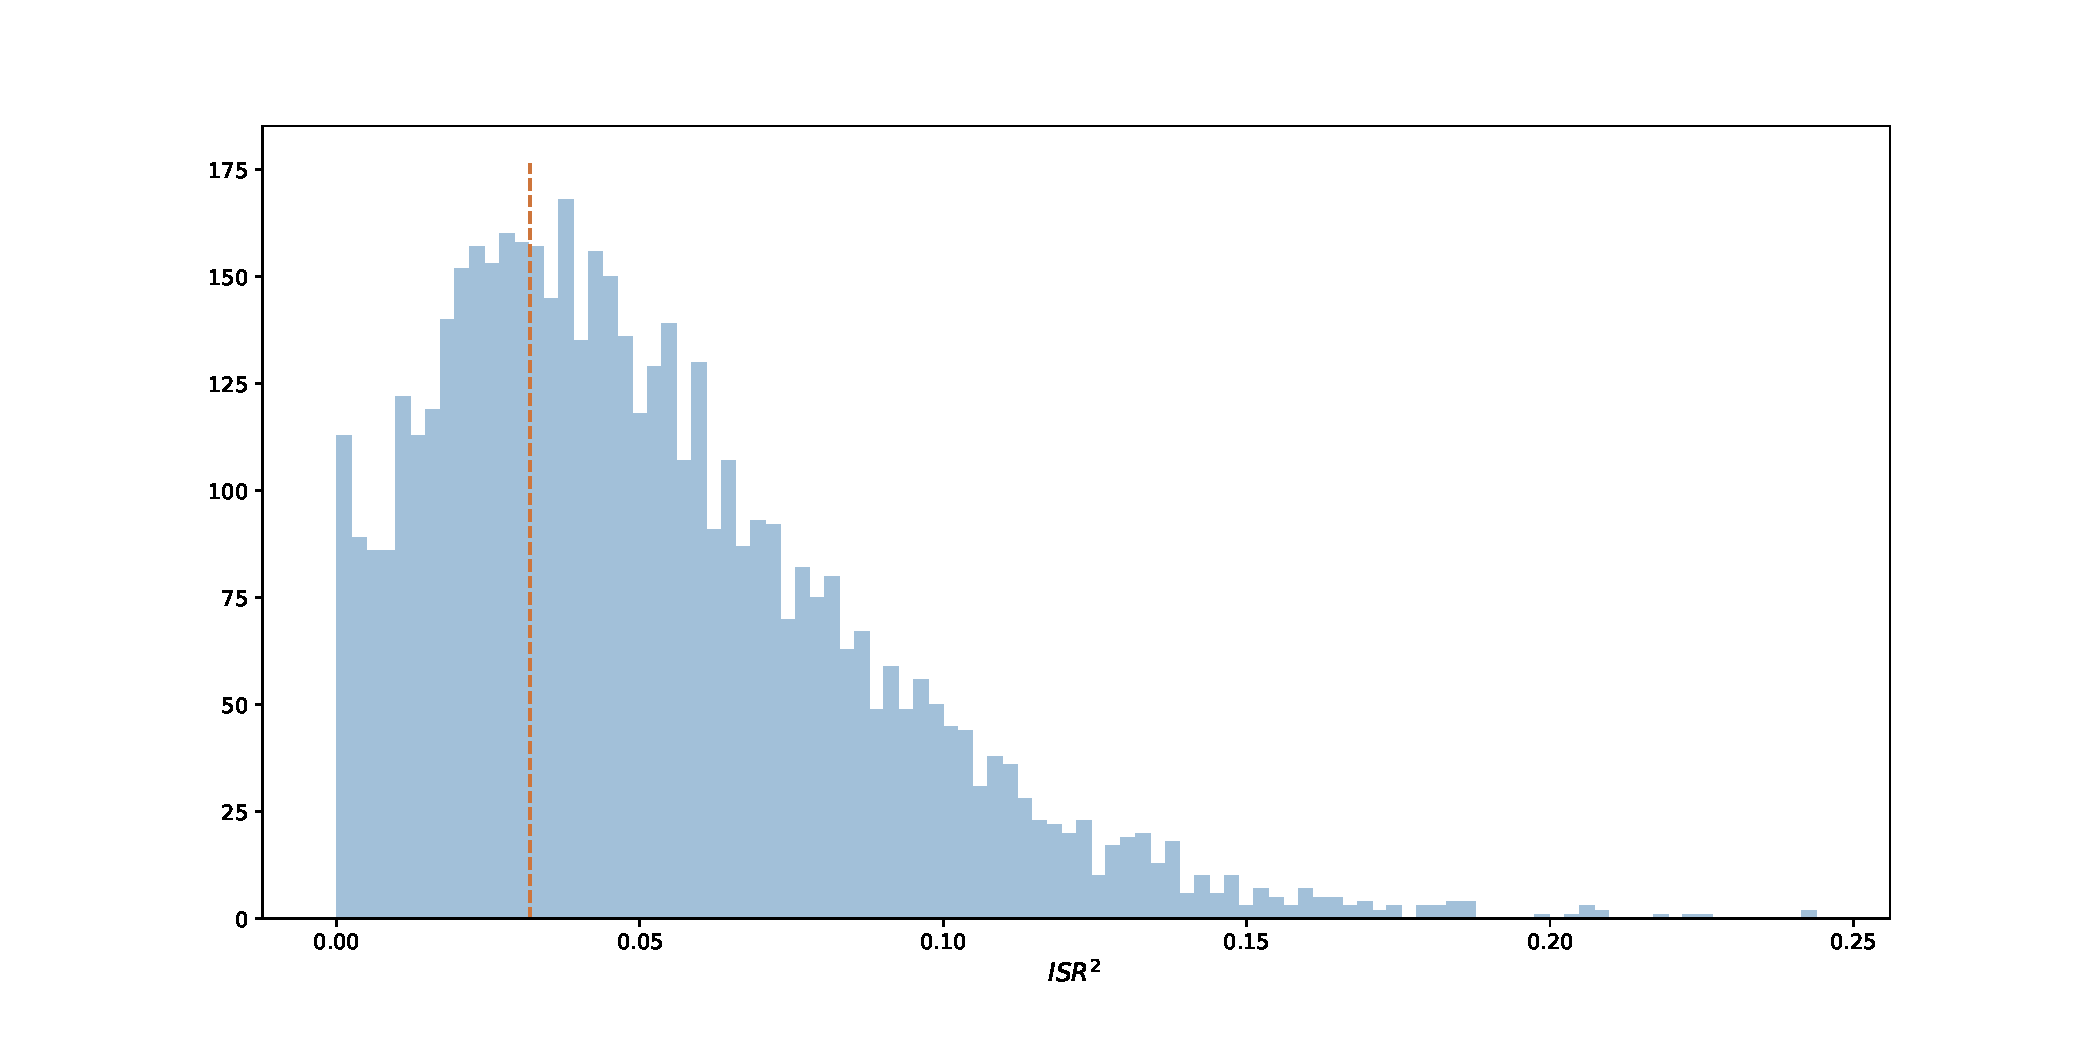
\includegraphics[width=\linewidth]{q4fig2.pdf}
\caption{This figure plots the distribution of in-sample $R^2$ under the null hypothesis. Our point estimate $0.032$ (dashed line) matches the distribution well. Hence we can not reject the null hypothesis.}
\end{figure}
\end{frame}

\begin{frame}{Q4: Simulation}
\begin{figure}[h!]
\centering
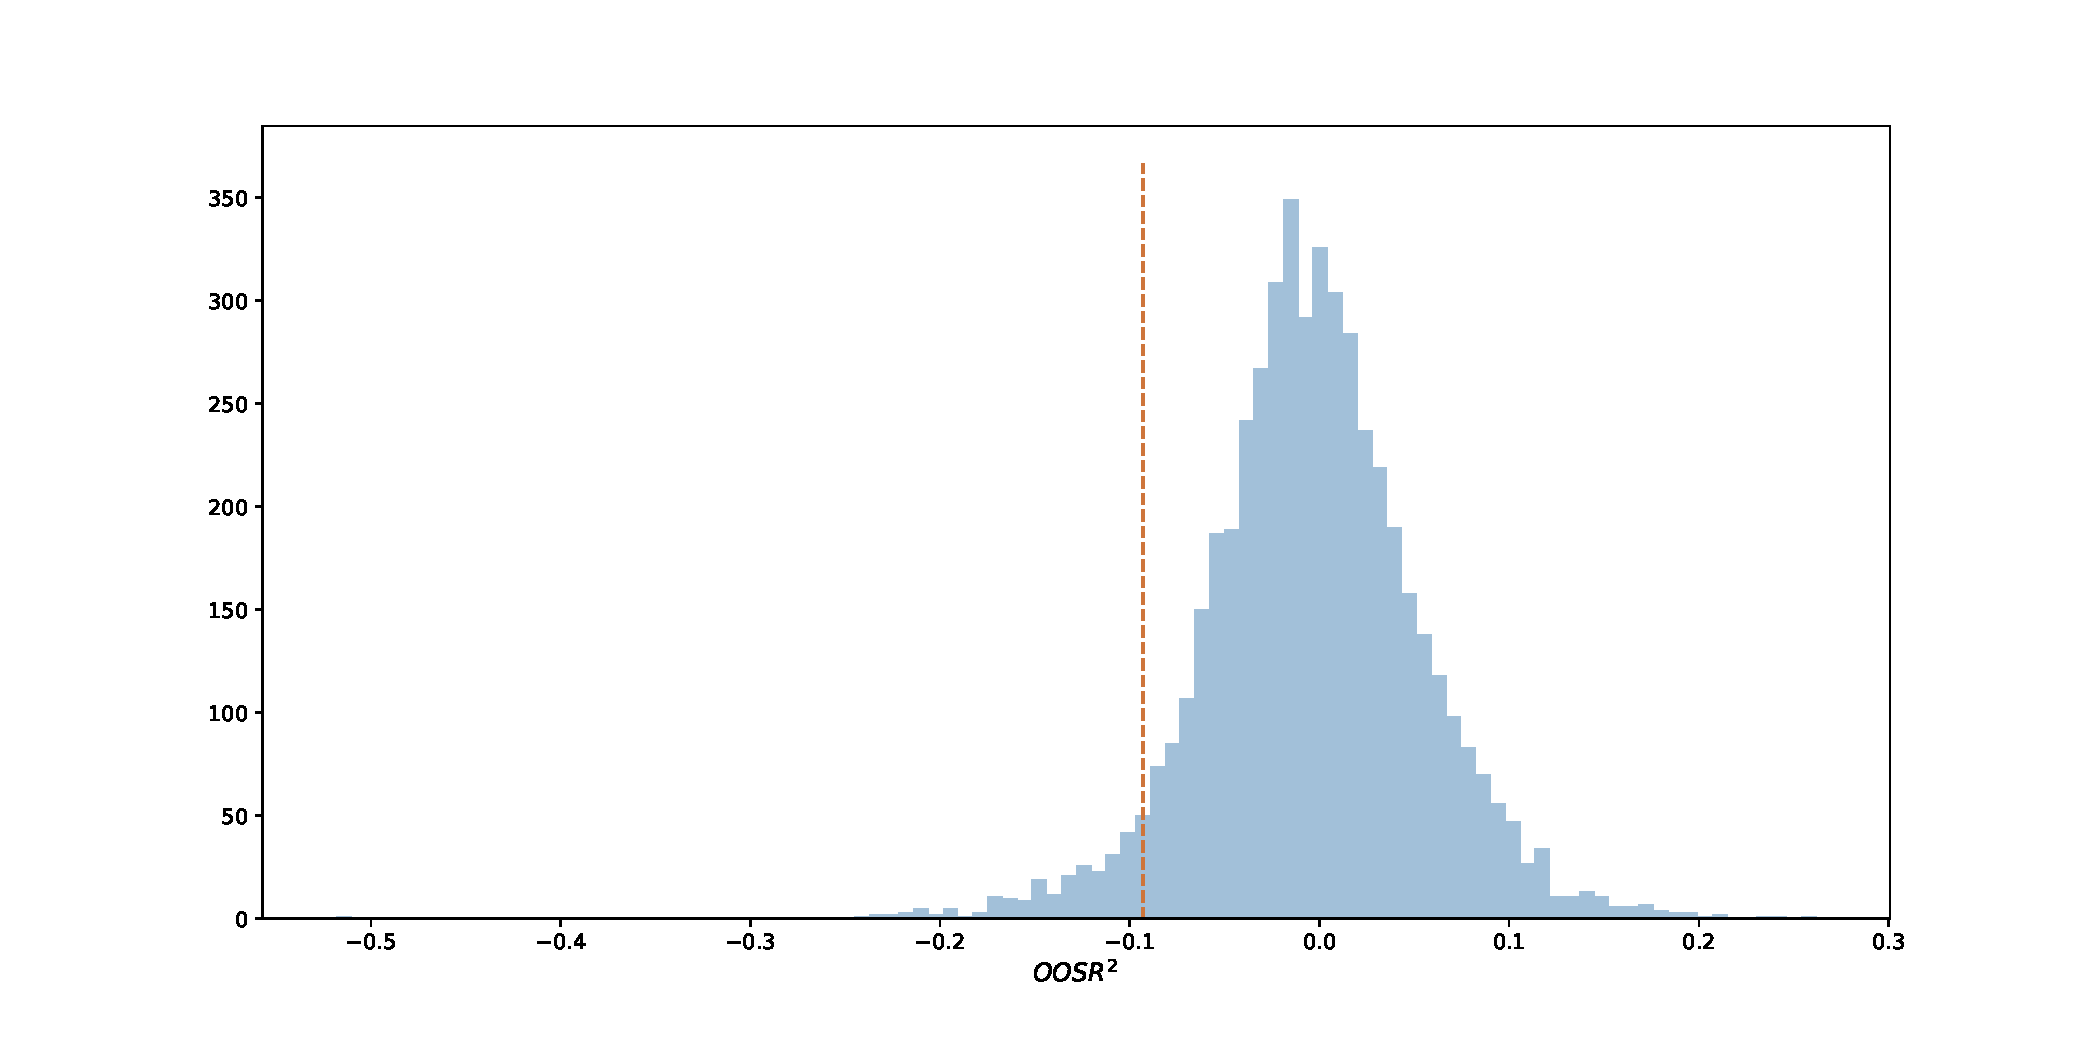
\includegraphics[width=\linewidth]{q4fig3.pdf}
\caption{This figure plots the distribution of out-of-sample $R^2$ under the null hypothesis. Our point estimate $-0.093$ (dashed line) lies at the left tail, but there still exists many simulated $OOSR^2$ lower than our sample estimate. Hence we can not reject the null hypothesis.}
\end{figure}
\end{frame}

\begin{frame}{Q4: Concluding remark}
\begin{itemize}
  \item The poor out-of-sample predictability implies that short-term (e.g., one-period) return is hard to predicted using fundamentals (e.g., $dp$). Short-term returns are quite volatile.
  \item However, this fact does not contradict against the long-term return predictability which says that time-varying risk premiums (or the long-term expected returns) dominate the variation in the stock price.
\end{itemize}
\end{frame}


\end{document}

